\documentclass{article}

\usepackage{a4wide}
\usepackage[utf8]{inputenc}
\usepackage[T1]{fontenc}
\usepackage[french]{babel}
\usepackage[babel=true]{csquotes} % guillemets français
\usepackage{graphicx}
\graphicspath{{Images/}}
\usepackage{color}
\usepackage{hyperref}
\hypersetup{colorlinks,linkcolor=,urlcolor=blue}

\usepackage{amsmath}
\usepackage{amssymb}


\title{Rapport de projet de jeu avec accéléromètre}
\author{\'Thomas Lenepveu, M1 informatique}
\date{\today}

\begin{document}

\maketitle % pour écrire le titre


%% Le résumé:
\begin{abstract}
  Dans ce rapport, il sera présenté un exemple simple d'application Android de type jeu vidéo, utilisant le capteur accéléromètre.
\end{abstract}

\section{Introduction}

Le but du projet a été de concevoir une application de type jeu vidéo pour Android. Cette application devait notamment implémenter:

\begin{itemize}
\item une activité de jeu dont le fonctionnement nécessite l'utilisation du capteur \textit{Accelerometer}
\item une gestion de scores permettant l'enregistrement des résultats des joueurs (y compris après fermeture du programme)  ainsi que leur affichage
\item la possibilité de cliquer sur un score et de visionner la localisation du joueur correspondant au moment où se score a été validé
\end{itemize}

\textit{NB: Au moment de la rédaction de ce document, l'interface des scores n'est pas finalisée et de ce fait les scores ne s'y affichent pas. Il reste toutefois possible d'afficher les scores sur Google Map et la vérification d'Intent nécessaire est implémentée (reste à coder l'envoi dynamique de cet Intent).}


\section{Application JeuAccelerometre}

\subsection{Structure du projet}
Le projet se décompose en 5 activités et une classe:
\begin{itemize}
\item une activité de démarrage StartActivity qui permet à l'utilisateur d'entrer son nom/pseudo, et d'accéder au choix à l'activité de jeu GameActivity ou à la page des scores ScoreActivity
\item une activité de jeu GameActivity qui est la partie de jeu en elle même: après 30 secondes d'activité, l'application bascule automatiquement à l'activité de jeu EndGameActivity
\item une activité de fin de jeu EndGameActivity qui capte la position du joueur et lui permet d'accéder à l'activité des scores ScoreActivity en enregistrant ou non son score courant.
\item une activité des scores ScoreActivity qui affiche les scores (non implémenté à la rédaction de ce document) en les lisant à partir d'un fichier, enregistre le nouveau score si nécessaire et permet d'afficher la page de carte ScoreMapActivity
\item une activité de carte ScoreMapActivity qui affiche l'ensemble des scores sur leurs positions respectives sur une carte Google Map
\item une classe serialisable ScoreData qui sert de classe de base pour enregistrer les données de score sur un fichier
\end{itemize}

\subsection{L'activité StartActivity}
L'activité StartActivity, comme son nom l'indique, est l'activité de démarrage de l'application. C'est un menu principal pour le joueur ou il peut entrer son nom/pseudo, lancer une partie ou entrer directement sur la page des scores. Si le joueur lance une partie, le champ texte correspondant à son nom/pseudo est passé dans l'Intent.
\begin{center}
  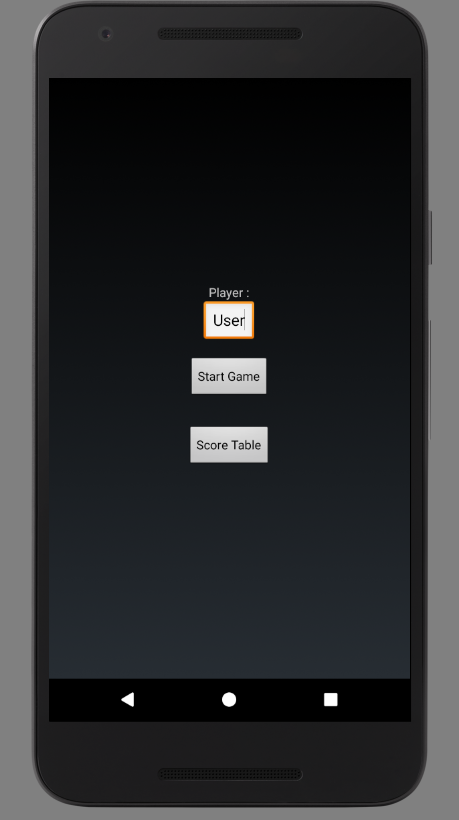
\includegraphics[scale=0.5]{StartActivity.png}
\end{center}

\subsection{L'activité GameActivity}
L'activité GameActivity est l'activité de jeu en tant que tel. Le système de jeu, fonctionnant par utilisation du capteur accéléromètre, est simple: tant que la balle est hors de collision avec les bords de l'écran, le joueur marque des points, sinon il en perd. La partie se termine après 30 secondes d'activité (la pause est gérée!) et bascule sur l'activité de fin de jeu EndGameActivity avec, dans l'Intent, le nom/pseudo du joueur et son score pour la partie courante.
\begin{center}
  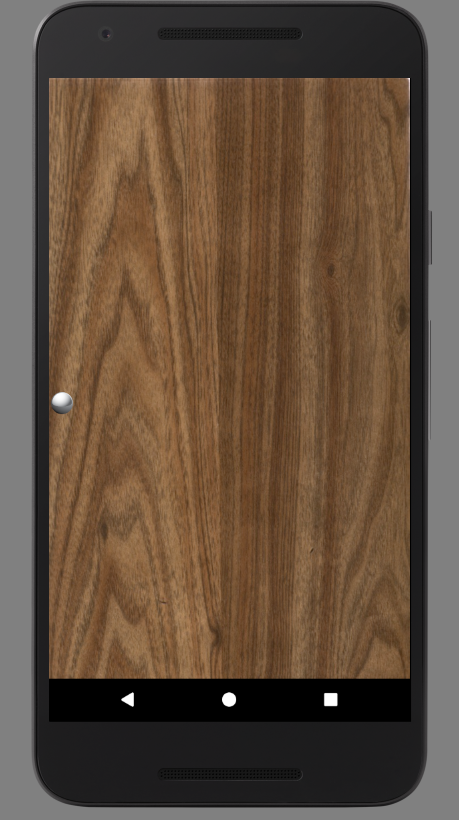
\includegraphics[scale=0.5]{GameActivity.png}
\end{center}
En particulier, le code de mise à jour de l'affichage est:
\textit{verbatim}:
\begin{verbatim}
protected void onDraw(Canvas canvas) {
            /*
             * Compute the new position of our object, based on accelerometer
             * data and present time.
             */
            final ParticleSystem particleSystem = mParticleSystem;
            final long now = System.currentTimeMillis();
            final float sx = mSensorX;
            final float sy = mSensorY;

            particleSystem.update(sx, sy, now);

            final float xc = mXOrigin;
            final float yc = mYOrigin;
            final float xs = mMetersToPixelsX;
            final float ys = mMetersToPixelsY;
            final int count = particleSystem.getParticleCount();
            for (int i = 0; i < count; i++) {
                /*
                 * We transform the canvas so that the coordinate system matches
                 * the sensors coordinate system with the origin in the center
                 * of the screen and the unit is the meter.
                 */
                final float x = xc + particleSystem.getPosX(i) * xs;
                final float y = yc - particleSystem.getPosY(i) * ys;
                particleSystem.mBalls[i].setTranslationX(x);
                particleSystem.mBalls[i].setTranslationY(y);
            }

            // and make sure to redraw asap
            invalidate();
        }
\end{verbatim}

\subsection{L'activité EndGameActivity}
L'activité EndGameActivity est entrée après 30 secondes de jeu: c'est sur cette activité que la localisation du jeueur est détectée. Le joueur peut décider d'entrer sur l'activité des scores ScoreActivity en enregistrant son score ou non: si oui, son nom/pseudo, score et position sous forme de latitude/longitude est passée dans l'Intent.
\begin{center}
  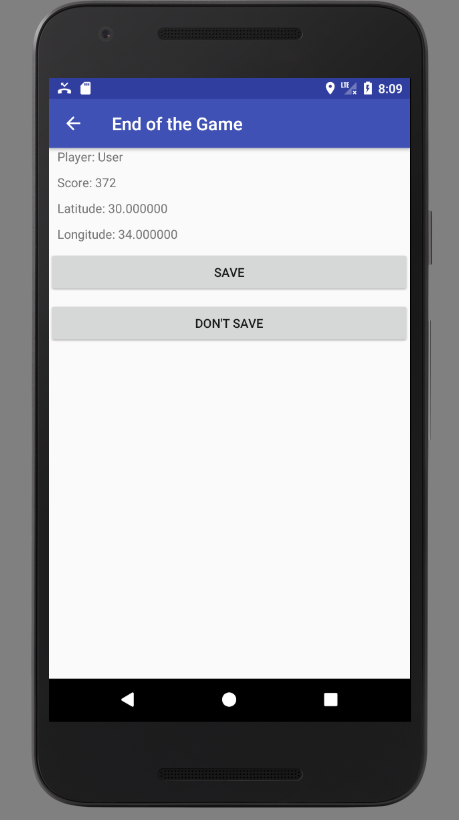
\includegraphics[scale=0.5]{EndGameActivity.png}
\end{center}
En particulier, la portion de code gérant l'écoute de capteur de localisation GPS est:
\textit{verbatim}:
\begin{verbatim}
		  try {
                            mFusedLocationClient.requestLocationUpdates(mLocationRequest,
                                    mLocationCallback, Looper.myLooper());
                        }catch(SecurityException e){

                        }
\end{verbatim}

\subsection{L'activité ScoreActivity}
L'activité ScoreActivity gère le chargement des scores à partir d'un fichier interne (implémenté) et l'affichage des scores (pas implémenté).Elle gère aussi l'enregistrement du nouveau score si elle est atteinte à partir de EndGameActivity avec demande d'enregistrement, en utilisant l'Intent transmis dans ce cas précis. Pour le moment, l'utilisateur peut accéder à la carte GoogleMap sur l'activité ScoreMapActivity par le biais d'un unique bouton.
\begin{center}
  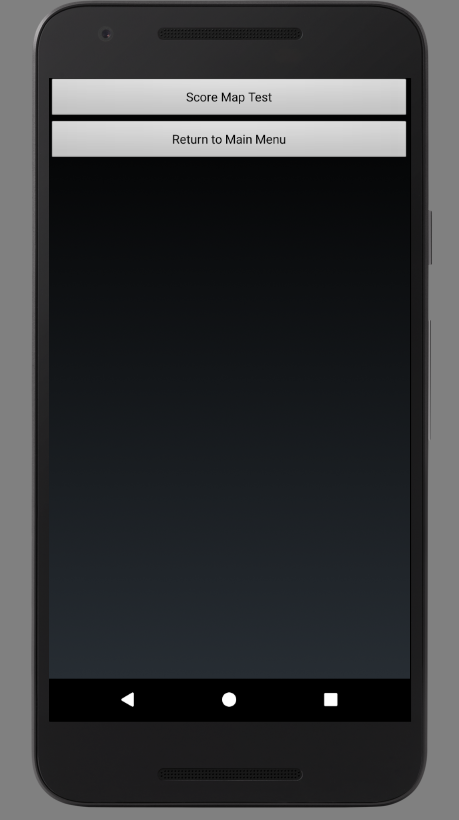
\includegraphics[scale=0.5]{ScoreActivity.png}
\end{center}
En particulier, la fonction d'écriture et de lecture de fichier (respectivement  par écriture sur un flux externe et lecture sur un flux interne) est implémentée de la manière suivante:
\textit{verbatim}:
\begin{verbatim}
public void saveScoreDataFile(){
        File d = getFilesDir();
        File f = new File(d, "ScoreDataFile.ser");
        FileOutputStream fos = null;
        try{
            fos = new FileOutputStream(f);
            ObjectOutputStream oos = new ObjectOutputStream(fos);
            oos.writeObject(score_list);
            oos.close();
            fos.close();
            System.out.println("Score list Save successful");
        }catch(Exception e){
            e.printStackTrace();
        }
    }
 public void loadScoreDataFile(){
        FileInputStream fis;
        try{
            fis = openFileInput("ScoreDataFile.ser");
            ObjectInputStream ois = new ObjectInputStream(fis);
            score_list = (ArrayList<ScoreData>) ois.readObject();
            ois.close();
            fis.close();
            System.out.println("Score list Load successful");
        }catch(Exception e){
            e.printStackTrace();
        }
    }
\end{verbatim}

\subsection{L'activité ScoreMapActivity}
L'activité ScoreMapActivity affiche une carte GoogleMap avec les positions des scores en jeu de chaque joueur. Il implémente le centrage sur une position de score donné si l'activité ScoreActivity lui transmet la latitude et longitude nécessaire.
\begin{center}
  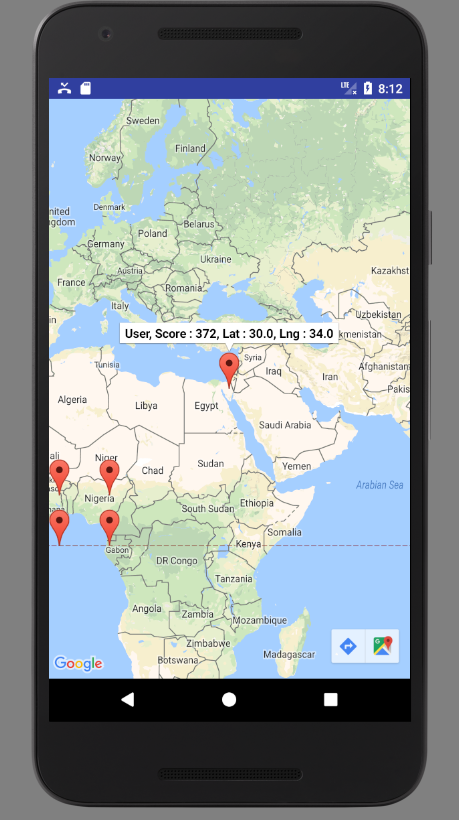
\includegraphics[scale=0.5]{ScoreMapActivity.png}
\end{center}
En particulier, l'affichage de chaque point-score sur la carte se fait avec la portion de code suivante:
\textit{verbatim}:
\begin{verbatim}
for(int i=0; i<score_list.size(); i++){
            mMap.addMarker(new MarkerOptions()
                    .position(
			new LatLng(
				score_list.get(i).getPlayer_lat(),
				score_list.get(i).getPlayer_lng()
			)
		)
                    .title(score_list.get(i).getPlayer_name()
                            + ", Score : " + score_list.get(i).getPlayer_score()
                            + ", Lat : " + score_list.get(i).getPlayer_lat()
                            + ", Lng : " + score_list.get(i).getPlayer_lng()
                    )
            );
        }
\end{verbatim}

\subsection{La classe ScoreData}
La classe ScoreData est une classe Serializable permettant l'anregistrement d'un nom/pseudo, d'un score, d'une latitude et d'une longitude. Elle sert aux classes ScoreActivity et ScoreMapActivity, en particulier à la classe ScoreActivity qui implémente la sauvegarde des scores dans un fichier.

\section{Conclusion}

Bien que le jeu en lui même soit simple et que l'interface des scores ne soit pas finalisée au moment de la rédaction de ce document, je suis, dans l'ensemble, assez satisfait du résultat de ce projet. Il s'agit de mon premier projet fonctionnel sous la plateforme Android, et je dois avouer que la gestion d'un nouvel environnement de développement (Android Studio) a été éprouvante. La gestion des mises à jour Gradle a été en particulier un problème récurrent. J'espère pouvoir finaliser l'interface des scores et rendre le jeu plus  intuitif (affichage en surbrillance du score en jeu) avant la présentation.

\end{document}
